\subsection{Background}
\label{uvm:sec:background}

\subsubsection{The GPU Memory Wall for LLM Inference}
\label{uvm:sec:bg:memwall}

Modern Large Language Model (LLM) inference workloads are increasingly
    constrained by GPU memory capacity.
The size of flagship LLMs has been growing
    at roughly $410\times$ every two years,
    while GPU memory capacity only doubles
    in the same period~\cite{ai-memory-wall}.
As a result, even high-end accelerators
    (e.g., A100 with $80$\,GiB or H100 with $80$\,GiB)
    struggle to host large models together with their working state.

LLM serving has two primary on-GPU memory consumers:
\begin{enumerate}
\item \textbf{Model weights}, whose size is fixed by the model architecture
    (e.g., tens to hundreds of GiB for $13$B--$70$B-parameter models);
\item \textbf{KV cache}, whose size grows linearly
    with sequence length and batch size~\cite{vllm}.
\end{enumerate}
To improve serving throughput,
    modern frameworks such as vLLM~\cite{vllm} batch concurrent requests.
Larger batches, however, inflate the KV cache
    and quickly exhaust GPU memory.

To cope, modern serving frameworks use CPU memory
    as a larger but slower memory pool
    and explicitly offload either part of the model weights~\cite{flexgen, vllm, infinigen}
    or part of the KV cache~\cite{flexgen, headinfer, hf-offload}
    when the working set exceeds GPU memory.
Each framework, however, re-implements its own offloading logic
    tailored to its own model and execution structure,
    leading to substantial engineering cost
    and limited reusability across the ecosystem.

\subsubsection{Unified Virtual Memory (UVM)}
\label{uvm:sec:bg:uvm}

Unified Virtual Memory (UVM) is a CUDA driver-level feature
    that lets GPU kernels access memory of the CPU and of peer GPUs
    transparently, without explicit programmer-managed copies.
On allocation through the \texttt{cudaMallocManaged} API,\footnote{Conventional GPU allocations use \texttt{cudaMalloc}, which allocates device-resident memory and does not support oversubscription.}
    pages are owned by the CUDA runtime
    and are migrated on demand between the CPU and GPU.
    % in response to GPU page faults
    % (or proactively via hints such as \texttt{cudaMemAdvise}
    % and \texttt{cudaPrefetchAsync}).

UVM is a natural systems-level answer to the GPU memory wall
    because it offers three properties that are otherwise
    laboriously re-implemented by every framework:
\begin{enumerate}
\item \textbf{Memory oversubscription.}
    UVM transparently spills data to CPU memory
    when GPU memory is full,
    enabling models larger than the physical GPU memory to run
    without CUDA out-of-memory (OOM) errors.
\item \textbf{Transparent data movement.}
    The driver migrates hot pages onto the GPU
    and can prefetch pages based on hints,
    avoiding hand-written \texttt{cudaMemcpy} pipelines.
\item \textbf{Unified memory access.}
    Both CPU and GPU can dereference the same virtual addresses,
    opening opportunities for hybrid CPU/GPU execution.
\end{enumerate}

On modern hardware with coherent CPU--GPU interconnects
    (e.g., NVLink-C2C on GH200, $\sim$$450$\,GB/s/dir),
    these properties become even more attractive:
    the high interconnect bandwidth makes CPU-resident accesses far cheaper.
    % the marginal cost of CPU-resident accesses drops sharply.


\subsubsection{Performance Gap of UVM}
\label{uvm:sec:bg:gap}

Despite its promise, UVM is widely regarded as too slow for production AI workloads.
PyTorch's documentation~\cite{pytorch-cuda-allocators} explicitly advises against
    using \texttt{cudaMallocManaged} for performance reasons,
    and prior work reports that UVM-based inference
    is over $5\times$ slower per request
    than application-level KV-cache offloading
    in FlexGen~\cite{flexgen, infinigen}.

We quantify the performance gap of UVM in \figurename~\ref{uvm:fig:motivation}.
We evaluate Hugging~Face OPT-13B inference on an H100 PCIe GPU across a range of batch sizes.
When the working set fits in GPU memory (\figurename~\ref{uvm:fig:motivation}a),
    vanilla PyTorch with its native \texttt{cudaMalloc}-based caching allocator (C1)
    is highly efficient.
In contrast, UVM (U0), implemented with PyTorch's \texttt{CUDAPluggableAllocator} interface, is $53\times$--$69\times$ slower than C1,
    and application-level KV-cache offloading (A) is $31\times$--$42\times$ slower
    due to the overhead of moving data over PCIe.
When we increase the batch size to oversubscribe the GPU memory (\figurename~\ref{uvm:fig:motivation}b),
    the native allocator (C1) crashes with an out-of-memory (OOM) error.
Application-level offloading (A) survives by explicitly moving the KV cache to host memory.
Naive UVM (U0) also survives, but its performance collapses:
    at batch size $40$, where the active working set exceeds GPU memory by $1.14\times$,
    UVM suffers from severe thrashing and becomes $5\times$ slower than application-level offloading.

\begin{figure}[H]
    \centering
    \begin{subfigure}[b]{\columnwidth}
        \centering
        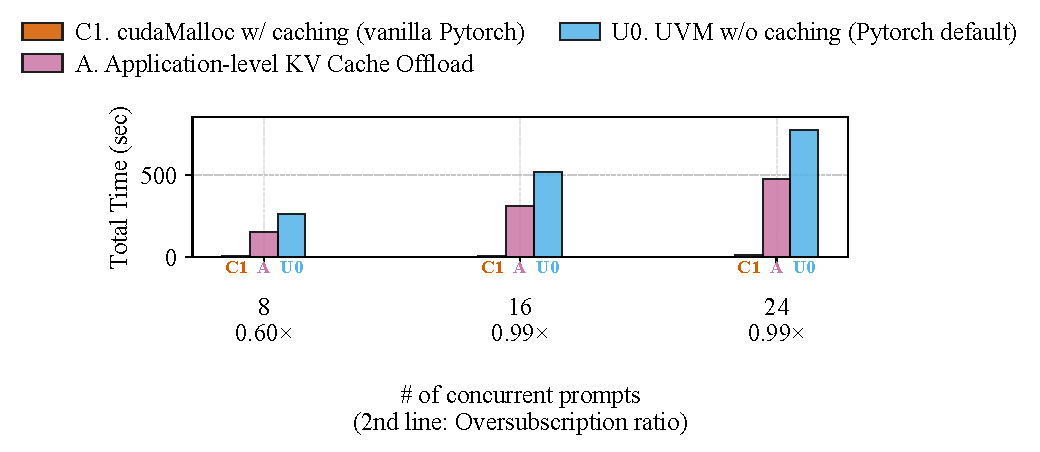
\includegraphics[width=\columnwidth]{figures/motivation_h100_small.pdf}
        \caption{Without oversubscription}
        \label{uvm:fig:motivation:small}
    \end{subfigure}
    \hfill
    \begin{subfigure}[b]{\columnwidth}
        \centering
        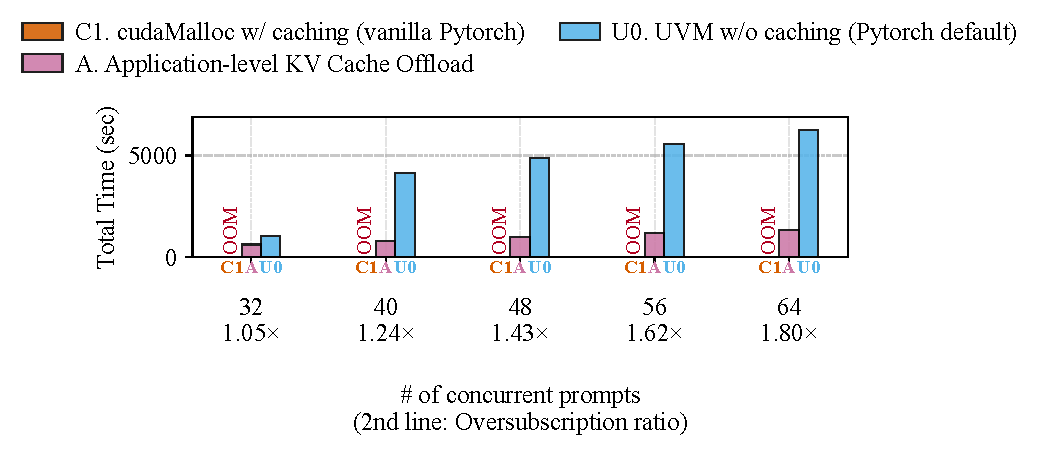
\includegraphics[width=\columnwidth]{figures/motivation_h100_large.pdf}
        \caption{With oversubscription}
        \label{uvm:fig:motivation:large}
    \end{subfigure}
    \caption{Performance gap of UVM for Hugging~Face OPT-13B inference on H100 PCIe.
        (a)~When the working set fits in GPU memory (batch sizes $8$--$24$),
        default UVM (U0) runs over $50\times$ slower than vanilla PyTorch (C1).
        (b)~When the GPU is oversubscribed (batch sizes $32$--$64$),
        UVM avoids OOM but thrashes,
        running up to $5\times$ slower than application-level KV-cache offloading (A).}
    \label{uvm:fig:motivation}
\end{figure}

We attribute this gap to two fundamental issues:

\paragraphb{Lack of application context}
The CUDA driver sees only a stream of memory accesses
    and has no insight into the structure of an LLM workload---%
    which tensors are weights versus activations,
    which blocks are about to be reused,
    or which blocks have been logically freed
    by the framework's own allocator.
As a result, UVM suffers long GPU page-fault handling latencies,
    redundant migrations,
    and pathological eviction decisions
    when the working set exceeds GPU memory.

\paragraphb{Inadequate framework support}
Modern AI frameworks such as PyTorch
    are built around their own caching allocators
    (e.g., the \texttt{CUDACachingAllocator} on top of \texttt{cudaMalloc}).
Using UVM with PyTorch today requires routing allocations through the
    \texttt{CUDAPluggableAllocator} interface,
    which bypasses this caching layer and allocates directly from the driver.
Every allocation and deallocation therefore reaches the driver,
    and each one must synchronize against all in-flight GPU kernels
    to avoid use-after-free errors,
    incurring substantial per-operation overhead.

Naively replacing \texttt{cudaMalloc} with \texttt{cudaMallocManaged}
    inside the caching allocator is not viable either.
The caching allocator relies on an allocation failure
    to trigger garbage collection and return memory to the driver,
    but \texttt{cudaMallocManaged} never fails---it simply spills to host memory.
A direct substitution therefore breaks this assumption,
    causing either host OOM kills or an unbounded UVM working set
    that destroys performance.

PyTorch has never built first-class UVM integration
    because UVM's degraded performance has left it impractical for production workloads.
To the best of our knowledge, our work is the first attempt
    to build a framework-aware UVM substrate for a production AI framework.
%     breaks key assumptions:
%     the allocator never returns memory to CUDA
%     (since \texttt{cudaMalloc} never appears to fail),
%     so the host kernel's OOM killer eventually terminates the process
%     long before UVM's spilling mechanism would naturally kick in.
% Vanilla UVM thus bypasses framework-level caching
%     while simultaneously breaking framework-level assumptions about residency.

% \subsubsection{PyTorch Memory Management}
% \label{uvm:sec:bg:pytorch}

% PyTorch manages GPU memory through its
%     \texttt{CUDACachingAllocator}~\cite{pytorch-cuda-allocators},
%     a user-space caching allocator built atop \texttt{cudaMalloc}.
% Two notions of memory are central to our discussion:
% \begin{enumerate}
% \item \emph{Active memory}: memory blocks
%     currently held by live PyTorch tensors and used in computation.
% \item \emph{Reserved memory}: memory the allocator has obtained from CUDA
%     and not yet released back.
% \end{enumerate}
% Reserved memory is typically larger than active memory because
%     (i)~the allocator retains freed blocks in its cache to amortize
%         \texttt{cudaMalloc} cost on future allocations, and
%     (ii)~a cached block may be partially reused
%         to satisfy a smaller request,
%         leaving the remainder fragmented but still pinned to the GPU.
% This caching policy is critical for performance
%     on \texttt{cudaMalloc} but,
%     as we show later,
%     interacts poorly with naive UVM
%     and creates the very fragmentation that motivates
%     {\uvmname}'s framework-guided eviction.

% \subsubsection{Modern Hardware: PCIe vs.\ Coherent Links}
% \label{uvm:sec:bg:hw}

% The cost of UVM page faults and migrations
%     depends strongly on the CPU--GPU interconnect.
% We consider three representative platforms in this work:
% \begin{enumerate}[leftmargin=*]
% \item \textbf{A100-PCIe} ($80$\,GiB device memory, PCIe Gen-4),
% \item \textbf{H100-PCIe} ($80$\,GiB device memory, PCIe Gen-4),
% \item \textbf{GH200} ($144$\,GiB device memory, NVLink-C2C).
% \end{enumerate}
% On the PCIe platforms, every page fault that misses on the GPU
%     triggers a costly migration over a relatively narrow link;
%     on GH200, the cache-coherent NVLink-C2C interconnect
%     makes CPU-resident accesses cheap enough that
%     the trade-off space for UVM shifts substantially.
% Understanding {\uvmname}'s behavior across this spectrum
%     is one of the contributions of this paper.
